\documentclass[]{article}

\usepackage[italian]{babel}
\usepackage[margin=20mm, footskip = 20pt]{geometry}
\usepackage{array}
\usepackage{tabularx}
\usepackage{graphicx}
\usepackage{subfiles}
\usepackage{hyperref}
\usepackage{nameref}
\usepackage{titlesec}
\usepackage{longtable}
\usepackage[table]{xcolor}
\usepackage{titling}
\usepackage{lastpage}
\usepackage{ifthen}
\usepackage{calc}
\usepackage{soulutf8}
\usepackage{contour}
\usepackage{float}
\usepackage{fancyhdr}
\usepackage{multirow}
\usepackage{pgfgantt}
\usepackage{lscape}

\newcommand{\hr}{\par\vspace{-.1\ht\strutbox}\noindent\hrulefill\par}

\graphicspath{ {./}
	{./commons/res}
}

%--------------------------------------------------
% Comandi per inserire contenuto del documento
%--------------------------------------------------
\makeatletter

\newcommand\appendToGraphicsPath[1]{%
	\g@addto@macro\Ginput@path{{#1}}%
}

\newcommand{\setTitle}[1]{%
	\newcommand{\@phTitle}{#1}%
}
\newcommand{\phTitle}{\@phTitle}

\newcommand{\setDate}[1]{%
	\newcommand{\@phDate}{#1}%
}
\newcommand{\phDate}{\@phDate}

\newcommand{\setUso}[1]{%
	\newcommand{\@uso}{#1}%
}
\newcommand{\uso}{\@uso}

\newcommand{\setVersione}[1]{%
	\newcommand{\@versione}{#1}%
}
\newcommand{\versione}{\@versione}

\newcommand{\disabilitaVersione}{%
	\renewcommand{\setVersione}[1]{}%
	\renewcommand{\versione}{DISABILITATA}
}

\newcommand{\setResponsabile}[1]{%
	\newcommand{\@responsabile}{#1}%
}
\newcommand{\responsabile}{\@responsabile}

\newcommand{\setRedattori}[1]{%
	\newcommand{\@redattori}{#1}%
}
\newcommand{\redattori}{\@redattori}

\newcommand{\setVerificatori}[1]{%
	\newcommand{\@verificatori}{#1}%
}
\newcommand{\verificatori}{\@verificatori}

\newcommand{\setModifiche}[1]{%
	\newcommand{\@modifiche}{#1}%
}
\newcommand{\modifiche}{\@modifiche}

\makeatother 

%--------------------------------------------------
% Comandi per i documenti esterni e il glossario
%--------------------------------------------------

\newcommand{\dext}[1]{\textsc{#1\textsubscript{\textit{D}}}}

\newcommand{\glock}[1]{\textsc{#1\textsubscript{\textit{G}}}}

%--------------------------------------------------
% Comandi per impostare sottotitoli di quarto e quinto livello
%--------------------------------------------------

\setcounter{secnumdepth}{4}
\setcounter{tocdepth}{4}

\titleformat{\paragraph}
{\normalfont\normalsize\bfseries}{\theparagraph}{1em}{}
\titlespacing*{\paragraph}{0pt}{2.25ex plus 1ex minus .2ex}{1.5ex plus .2ex}

\titleformat{\subparagraph}
{\normalfont\normalsize\bfseries}{\thesubparagraph}{1em}{}
\titlespacing*{\subparagraph}{0pt}{1.75ex plus 1ex minus .2ex}{.75ex plus .1ex}

\appendToGraphicsPath{../../../commons/res/}

%------------------------------
%
% COMANDI DI CONFIGURAZIONE
%
%------------------------------

\setTitle{Verbale esterno \#4}

\setVersione{1.0.0}

\setDate{23-02-2021}

\setResponsabile{Lucia Fenu}

\setRedattori{Alessandro Dindinelli}

\setVerificatori{Giacomo Bulbarelli}

\setUso{Esterno}

\setModifiche{
	1.0.0 & Lucia Fenu & Responsabile & 13-03-2020 & Approvazione documento\\
	0.1.0 & Giacomo Bulbarelli & Verificatore & 10-03-2021 & Verifica prima stesura\\
	0.0.0 & Alessandro Dindinelli & Amministratore & 23-02-2021 & Stesura iniziale}

\begin{document}

	% Direttive per la creazione del titolo tramite comando maketitle
\title{\huge \textsc{\phTitle{}} \\
	\vspace{11pt} \large \textsc{\phDate{}}}

\author{} % Non toccare
\date{} % Non toccare

%--------------------
% Frontespizio
%--------------------

% Logo del gruppo
\begin{figure}[t!]
	\centering
	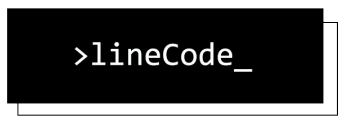
\includegraphics[width=20em]{lclong}
\end{figure}

% Titolo / Nome
\maketitle
\thispagestyle{empty}

% Dati specifici sul doc in forma tabulare
\begin{table}[ht]
	\begin{center}
		\label{tab:Dati sul documento}
		\begin{tabular}{r|l}
			\multicolumn{2}{c}{ \textsc{Dati sul documento} } \\
			\hline
			\textbf{Versione} & \versione{} \\
			\textbf{Uso} & \uso{}  \\
			\textbf{Redattori} & \redattori{} \\
			\textbf{Verificatori} & \verificatori{} \\
			\textbf{Responsabile} & \responsabile{} \\
			\textbf{Destinatari} & lineCode \\
								& prof.\ Vardanega Tullio \\		
								& prof.\ Cardin Riccardo \\
			\ifthenelse{\equal{\uso}{Esterno}}{
								& Sanmarco Informatica
			}{} \\
		\end{tabular}
	\end{center}
\end{table}

\newpage

\renewcommand{\arraystretch}{2} % allarga le righe con dello spazio sotto e sopra
\begin{longtable}[H]{>{\centering\bfseries}m{2cm} >{\centering}m{3.5cm} >{\centering}m{2.5cm} >{\centering}m{3cm} >{\centering\arraybackslash}m{5cm}}
	\rowcolor{lightgray}
	{\textbf{Versione}} & {\textbf{Nominativo}} & {\textbf{Ruolo}} & {\textbf{Data}} & {\textbf{Descrizione}}  \\
	\endfirsthead%
	\rowcolor{lightgray}
	{\textbf{Versione}} & {\textbf{Nominativo}}  & {\textbf{Ruolo}} & {\textbf{Data}} & {\textbf{Descrizione}}  \\
	\endhead%
	\modifiche{}%
\end{longtable}

	\newpage

	%--------------------------------
	%
	% IL CONTENUTO INIZIA DA QUI
	%
	%--------------------------------

	\section{Introduzione}
		\subsection{Luogo e data dell'incontro}
		\begin{itemize}
			\item \textbf{Modalità}: Telematica;
			\item \textbf{Software utilizzato}: Google Meet;
			\item \textbf{Data}: 23 Febbraio 2021;
			\item \textbf{Ora di inizio}: 11:00;
			\item \textbf{Ora di fine}: 12:00.
		\end{itemize}

		\subsection{Presenze}
		\begin{itemize}
			\item \textbf{Presenti}:
			\begin{itemize}
				\item Matteo Alba
				\item Giacomo Bulbarelli
				\item Alessandro Chimetto
				\item Alessandro Dindinelli
				\item Paolo Scanferlato
			\end{itemize}
			\item \textbf{Assenti}:
			\begin{itemize}
				\item Lucia Fenu
				\item Valton Tahiraj
			\end{itemize}
			\item \textbf{Partecipanti esterni}:
			\begin{itemize}
				\item Alex Beggiato (referente, SanMarco Informatica)
			\end{itemize}
		\end{itemize}

		\subsection{Ordine del giorno}
		\begin{enumerate}
			\item Tecnologie consigliate;
			\item microservizi;
			\item ridondanza componente grafica;
			\item containers;
			\item database;
			\item architettura dei mock;
			\item sicurezza.
		\end{enumerate}
\newpage
	\section{Svolgimento}
	L'incontro è servito al gruppo per confrontarsi con il referente di SanMarco Informatica, riguardo alcuni dubbi sorti durante lo studio delle tecnologie con cui si dovrà lavorare.

		\subsection{Tecnologie consigliate}
		Per lo sviluppo di servizi RESTful sono stati proposti alcuni possibili framework, da cui poi il referente ha consigliato di appoggiarsi ad uno dei seguenti:
		\begin{itemize}
			\item \textbf{\glock{Jersey}}: semplice da comprendere, è specializzata in questo tipo di servizi, il che renderebbe semplice un cambio di tecnologia qualora ce ne fosse bisogno;
			\item \textbf{\glock{Spring}}: soluzione più complessa, svolge le funzioni di \glock{Jersey} ma offre maggior integrazione con \glock{Java} e permette più funzionalità.
		\end{itemize}
		Per quanto la crezione della mappa, nel caso più semplice di un prototipo potrebbe bastare una tabella in \glock{html} resa più appetibile tramite \glock{css}; all'aumentare della complessità è stato consigliato l'utilizzo di \glock{d3js}.

		\subsection{Microservizi}
		Era sorto il dubbio che il tipo di architettura che si svilupperà potesse ricondursi ad un'architettura a microservizi. Si è chiarito che è sconsigliato un approccio di questo tipo, in quanto le componenti che andranno a comporre il sistema non saranno eccessivamente numerose.

		\subsection{Ridondanza componente grafica}
		Riguardo il requisito che prevede di garantire \glock{zero-downtime} all'applicazione, è stato deciso che non è necessario avere una ridondanza anche della componente grafica del sistema. Nella pratica si garantisce l'affidabilità sul core, cioè che può creare problemi in caso di sua assenza, ma il monitor non presenta tale criticità.

		\subsection{Containers}
		Durante lo studio di \glock{Docker}, si è discusso di tecnologie affini come \glock{Kubernetes}. Un tale approccio è stato giudicato eccessivo, considerando più adatto l'utilizzo di \glock{docker-compose}.

		\subsection{Database}
		I dati che l'applicazione richiede consistono principalmente dell'anagrafica degli utenti e delle unità. Essendo dati con i quali non si interagirà molto, ma che sono di grande importanza, è stato consigliato di salvarli direttamente in un database, evitando una soluzione in memory.

		\subsection{Architettura dei mock}
		Per testare le funzionalità dell'applicazione, soprattutto nelle fasi iniziali, è stato consigliato di avere una mappa con struttura a scacchiera. Inoltre si consiglia, quando viene generato un ostacolo, di inviarne la posizione alle unità in base alla loro distanza dall'ostacolo stesso. Tale implementazione dipenderà comunque da come verrà sviluppato il motore di calcolo.

		\subsection{Sicurezza}
		Usare le best practices, comunicando con https, usando anche un certificato auto-generato. Salvare l'hash delle password nel database, in modo da garantire maggiore sicurezza.

	\newpage

	\section{Tabella delle decisioni}

\begin{table} [h!]
	\rowcolors{2}{gray!25}{gray!6}
	\begin{center}
		\begin{tabular} { m{2cm} m{14cm} }
			\rowcolor{lightgray}
			\textbf{ID} & \textbf{Decisione}\\
			VE_2021-02-23_4.1 & Come libreria di servizi RESTful, si è consigliato di scegliere tra \glock{Jersey} e \glock{Spring}.\\
			VE_2021-02-23_4.2 & Non è necessario garantire ridondanza per la componente grafica del sistema.\\
			VE_2021-02-23_4.3 & Raccomandato l'utilizzo di \glock{docker-compose}, rispetto ad altre soluzioni di container.\\
			VE_2021-02-23_4.4 & Raccomandato l'utilizzo di un database relazionale, non in memoria, per l'anagrafica degli utenti e delle unità.\\
			VE_2021-02-23_4.5 & Salvare l'hash delle password nel database.
		\end{tabular}
	\end{center}
\end{table}
\end{document}

